\chapter{Parallel computing}\label{ch:gpu}
Ever since the chip manufacturing industry stopped increasing significantly the frequency of operation of the processing units and, instead, included an ever increasing number of computational \textit{cores}, the only way to fully exploit the performance of the newest hardware is the way of the parallelism.\\
A parallel execution of a program is able to perform several computations, independent from each other, at the same time usually called \textit{threads}. If a \textit{multi-core} processing unit is available, each core is able to process one of the computation at the same time another core is executing its task. However, there are factors that complicates the writing of a functioning parallel program, for instance there is no guarantee in the order of execution of the different threads and, if one depends upon the result of another, that must be taken into account.\\
In the following section we will give a brief overview of the most important principles of parallel computing.

\section{Principles of parallel computing}
Traditionally software has been written for serial execution. Which means that the series of instructions to be performed to execute a program are evaluated one by one, always in the same order. This approach requires that for hardware to execute a given program faster the time to evaluate a single instruction must be made shorter, and since a processing unit evaluates an instruction at every \textit{clock cycle}, the overall frequency has to increase.\\
From the first microprocessor up to the early years 2000s the increase in frequency was indeed the driving factor in the improvement of the performance of sequential software. However, when processors hit the higahertz domain, it became apparent that the continuous increase in frequency could not hold for long as it required at the same time an increase in the power required to operate the processing units, which also meant bigger and more complex systems to dissipate the resulting heat produced.\\
At the same time, nevertheless, the manufacturing was still able, year after year, to reduce the size of the transistors inside the chip. Thus the first \textit{dual core} processor was born: including two processing cores able to perform arithmetic operations independently while accessing the data from a common memory.\\

\subsection{Moore's law}
In 1965 Gordon Moore, Intel co-founder, stated that the number of transitor on integrated circuits doubles about every two years \cite{moore}. Figure \ref{moore} shows that since the early '70 until today the law has proven to be quite accurate.

\begin{figure}
\includegraphics[width=0.8\textwidth]{architectures/moores.png}
\caption{Number of transistor count in logarithmic scale with respect to the year of introduction. Credit to \href{https://commons.wikimedia.org/wiki/User:Wgsimon}{Wgsimon}, \href{http://creativecommons.org/licenses/by-sa/3.0/}{CC BY-SA 3.0}}
\label{moore}
\end{figure}
\clearpage

\subsection{Amdahl's Law}
With multi-core processor available we can now parallelize a program to split up the load on as many cores available, therefore one could expect, for an eight core machine for instance, to have an increase in performance of a factor eight. Unfortunately that is not the case: in every parallel program there is always a fraction of execution that has to be performed sequentially limiting the overall gain in performance, this limit takes the name of \textit{Amdahl's Law} \cite{amdahl}.\\
Let $T_S$ be the execution time of a sequential program, while $T_p$ the execution time of a program performing the same task of the sequential one but in parallel over $p$ processing units. The \textit{speedup} is then defined as the ratio $S(p) = \dfrac{T_S}{T_p}$.
Let $f$ be the fraction of the program running sequentially, the execution time of the parallel program is then $f T_S + (1 - f) T_p = f T_S + \dfrac{(1-f)T_S}{p}$. Which we can now substitute in the speedup formula to obtain its dependency with the fraction $f$ of sequential execution:
\begin{equation}
S(p,f) = \dfrac{T_S}{f T_S + \dfrac{(1-f)T_S}{p}}
\end{equation}
From which it is clear that even with an infinite number of parallel units there is a hard limit on the maximum obtainable speedup, indeed:
\begin{equation}
S_{max} \equiv \lim_{p\to\infty} S(p,f) = \dfrac{1}{f}
\end{equation}
As an example consider a program where only $5\%$ of its execution is sequential, the maximum speedup possible according to Amdahl's Law is then $S_{max} = \dfrac{1}{0.05} = 20$.
Figure \ref{amdahl} shows the maximum speedup obtainable for different values of $f$ as a function of $p$.

\begin{figure}
\centerline{\includegraphics[width=0.8\textwidth]{architectures/amdahl.png}}
\caption{Maximum theoretical speedup for various values of $f$ as a function of the number of parallel processes. Credit to \href{https://en.wikipedia.org/wiki/User:Daniels220}{Daniels220}, \href{http://creativecommons.org/licenses/by-sa/3.0/}{CC BY-SA 3.0}}
\label{amdahl}
\end{figure}

\section{Architectures}\label{sec:gpu_arch}

The architectures of a CPU and a GPU differs greatly. While the CPU focus on having few but very complex computational cores equipped with a large pool of memory, the GPU, on the other hand, has thousands of very simple cores that have to share a minimal amount of memory. Figure \ref{archs} shows a simplified scheme of the most usual architectures of a CPU and a GPU.

\begin{figure}
\centerline{\includegraphics[width=0.8\textwidth]{architectures/archs.png}}
\caption{a) Scheme of a CPU where most of the transistors are dedicated to caches and control unit. b) Scheme of a GPU with most of the resources used for the numerous execution units.}
\label{archs}
\end{figure}

\subsection{CPU architecture}
The main goal of the CPU design is to optimize the instruction execution latency, in order to achieve that there are some key design techniques:
\begin{itemize}
\item \textbf{Large cache memories} These memories are designed to reduce the data access time by keeping as many useful data as possible thus reducing the need to access the DRAM which, by comparison, is much slower.
\item \textbf{Complex control unit} This unit performs several evaluations in order to increase the efficiency of the CPU. Among those two are fundamental: \textbf{Branch prediction}, the control unit tries to guess the result of a branch in the code (e.g. an if-then-else statement) and fetch the data for that path before the branch is executed. \textbf{Operand forwarding} takes place when an operation needs the result of the previous one, in this case the operand forwarding bypass the write/read of the data into a register and simply pass it to the next operation, saving two CPU cycles and avoiding the stall of the second operation during those cycles.
\item \textbf{Powerful Arithmetic Logic Units (ALUs)} Beyond the most common arithmetic operations (sum, subtraction, etc...) most recent CPU's ALUs can perform much more complex operations in a single clock cycle, like, for instance, summing two vectors of 128 bits each.
\end{itemize}

\subsection{GPU architecture}
The GPU is, instead, designed to have a high \textit{throughput} of instructions, that is to perform a high number of instructions at the same time. The main design features oriented toward this results are:
\begin{itemize}
\item{As many ALUs as possible} The whole point of the GPU architecture is to have the highest amount of simple ALUs so that many simple operations can be performed at the same time.
\item{Simple control unit} Neither branch prediction nor operand forwarding are available. Branches are instead predicated meaning that all the branches are translated in machine code and only the active branch is executed while the other one is idling.
\item{Small caches} Caches are just used to stage the memory before execution preventing the ALU to access directly the DRAM.
\end{itemize}

In this work we focus on the GPUs manufactured by NVIDIA and programmed through the APIs called \textit{Compute Unified Device Architecture} (CUDA).
Figure \ref{kepler} shows the general layout of a NVIDIA Kepler architecture, similar to that used throughout most of this work.

\begin{figure}
\centerline{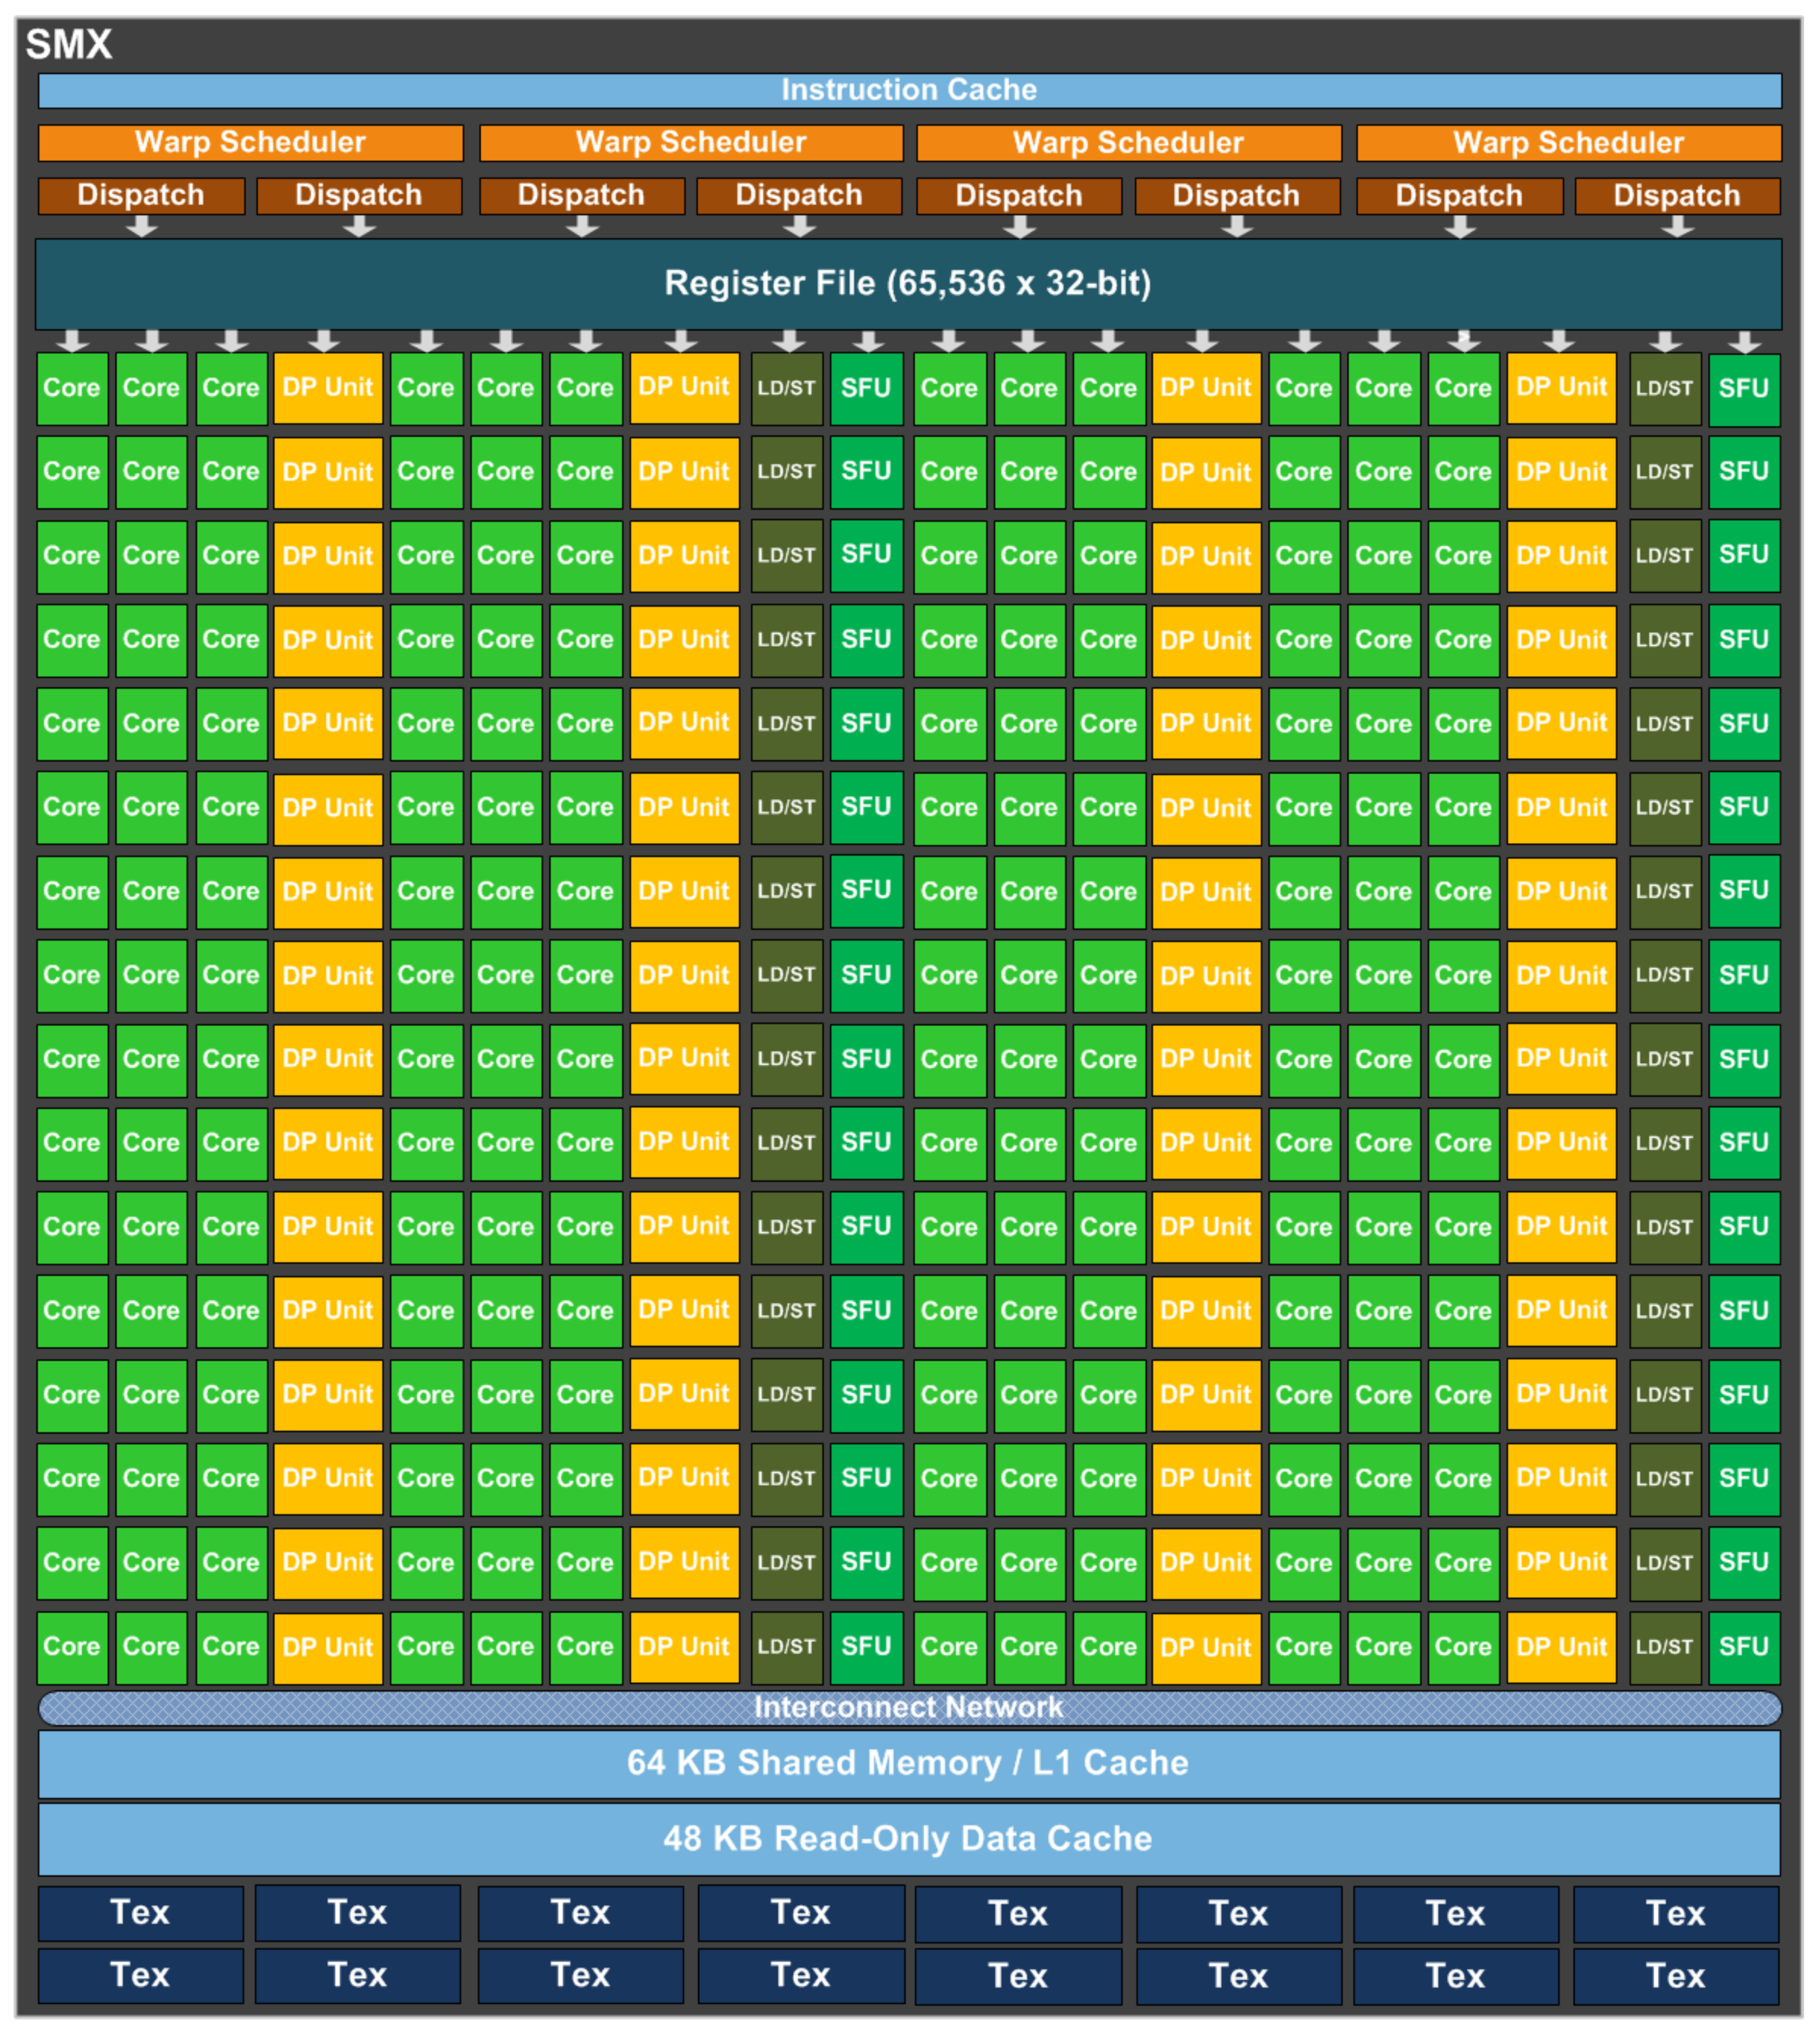
\includegraphics[width=0.9\textwidth]{architectures/kepler.png}}
\caption{A NVIDIA Kepler GPU equipped with 192 single-precision CUDA cores.}
\label{kepler}
\end{figure}

\section{CUDA C}
CUDA C is a set of extensions to the C programming language that allows to organize the execution of a program on a NVIDIA GPU.
The CUDA programming model establish two separate memory spaces: the \textit{host memory} that is the space of the computer hosting the GPU device and the \textit{device memory} which is the DRAM that only the GPU has direct access to.\\
The general concept of a CUDA program is that it starts with a serial code executing on the host machine that sets up the parallel code which then is executed in a large number of threads on as many GPU cores. When the GPU elaboration ends the control goes back to host where the data is gathered from the device and the program terminates.

\subsection{Threads and Memory Hierarchy} 
In order to fully profit of the high number of cores of a GPU it is necessary to have a tight control on the generation and coordination of the threads.
To fullfil this need CUDA organizes the groups of threads that can cooperate in \textit{blocks} and the set of all blocks in a single \textit{grid}.
Therefore every thread has an index representing its position inside its block and an index representing the position of its block in the grid.
Knowing those two indices and the dimension of the block each thread knows its absolute index with respect to the whole grid, knowing exactly which part of the parallel task to perform.
The reason behind the grouping of the threads in blocks which are subset of the grid is the memory hierarchy of the GPU. As a matter of fact the memory available on the GPU is organized in three groups of different size, visibility, lifetime and access time. Table \ref{tabMemory} presents the main characteristic of the memory types available in a NVIDIA GPU, with the sizes of the Teska k40 for reference.

\begin{center}
\begin{table}[h]
\begin{tabular}{ l | l | l | l | l}
\textbf{Memory} & \textbf{Visibility} & \textbf{Lifetime} & \textbf{Access time} & \textbf{Size (k40)}\\
\hline
Registers & Thread & Thread & Very fast & 90 Bytes \\
Shared mem. & Block & Block & Fast & 48 kBytes \\
Global mem. & Grid & Application & 150 $\times$ slower than SM & 12 GB \\
\end{tabular}
\caption{Characteristics of the memories in a typical NVIDIA GPU and sizes of the Tesla k40 for reference.}
\label{tabMemory}
\end{table}
\end{center}

\subsection{Memory management}
CUDA requires from the user to explicitly indicate the area of memory on the host where the data will be taken from and the area where the output will be saved on the host.
It also requires from the user to request the global memory space on the device that needs to be allocated for the process to be executed.
To accomplish those requirements CUDA provides the following functions to manage the memory on the device:
\begin{itemize}
\item \textbf{cudaMalloc()} Works similarly to the C malloc() function allocating a given size of memory in the device global memory addressed by the pointer passed as argument to the function.
\item \textbf{cudaFree()} Frees the global memory at the address passed as argument making it available again.
\item \textbf{cudaMemcpy()} Takes as arguments the address of a memory area on the host and that of an area in the device, the size of the transfer and then the direction the transfer should be made: \textbf{hostToDevice} to copy the data from the host to the GPU, \textbf{deviceToHost} to copy the data from the GPU to the host.
\item \textbf{cudaMemcpy()} Works exactly as the former but asynchronously, that is the CPU is free to perform the next instruction while the memory copy to/from the GPU is undergoing.
\end{itemize}

\subsection{Streams}
Most recent NVIDIA GPUs are able to perform three operations at the same time:
\begin{itemize}
\item memory copy from the host to the device
\item threads execution 
\item memory copy from device to host
\end{itemize}
 To fully exploit this feature the whole GPU execution must be divided in \textit{streams}. Each stream performs the three operation sequentially, however different streams can interleave each operation in order to maximise the occupancy of the calculation cores and the memory copy engines. Figure \ref{streams} shows a scheme of how two streams could interleave.

\begin{figure}
\centerline{\includegraphics[width=0.9\textwidth]{architectures/streams.png}}
\caption{Example of two CUDA streams execution.}
\label{streams}
\end{figure}
\newpage

\section{Testing hardware}\label{sec:benchmark}
The Research $\&$ Development of this work has been performed mainly on a workstatation equipped with a recent CPU and a NVIDIA Tesla k40c.
The relevant specification of the important hardware of the benchmark machine are reported below:
\begin{itemize}
\item \textbf{CPU} Intel i7-3770 - Max frequency: 3.9 $\unit{GHz}$, cores: 4, cache: 8 $\unit{MB}$
\item \textbf{System memory} DDR3 - size: 8 $\unit{GB}$, frequency: 1600 $\unit{MHz}$
\item \textbf{GPU} NVIDIA Tesla k40c - Max frequency: 850 $\unit{MHz}$, CUDA cores: 2880, onboard GDDR5 size: 12 $\unit{GB}$
\end{itemize}